\documentclass[10pt,handout]{beamer}

\usetheme[tuw_frametitletotop]{tuw}
\setbeamertemplate{footline}{}

\usepackage{lmodern}
\usepackage[utf8]{inputenc}
\usepackage{listings}
\usepackage{booktabs}
\usepackage{url}
\usepackage[style=ieee]{biblatex}
\usepackage{animate}
\usepackage{graphicx}
\usepackage{subcaption}
\usepackage[linesnumbered,ruled,vlined,resetcount]{algorithm2e}
\addbibresource{content/references.bib}
\renewcommand*{\bibfont}{\scriptsize}     %%attributes the footnotesize to the bibliography font.

%%% title page settings
\title[Seminar on Algorithms]{%
  184.754 Seminar on Algorithms 
}
\subtitle{Paper: Coloring the Vertices of 9-pt and 27-pt Stencils
with Intervals \\
\null
Supervisor: Prof. Dr. Jesper Larsson Träff}
\author{Camilo Tello Fachin}
\date{\today}

%%% slides start here
\begin{document}

% first frame must include the title page!
\begin{frame}
  \titlepage
\end{frame}

% table of contents if you have a long presentation (uses 'part' and 'section'
% elements)
\begin{frame}{Outline}
  \tableofcontents
\end{frame}

\section{Introduction}

\begin{frame}{Intro Slide}
    Still to do..
\end{frame}

\section{Interval Vertex Coloring (IVC)}
  \begin{frame}[fragile]
    hi there
  \end{frame}

  \subsection[Paragraphs]{Simple Paragraphs}
  \begin{frame}[fragile]
    \frametitle{Title first category}
    \framesubtitle{Title second category}
    % no deeper title hierarchy provided
  
    Lets see if the citation works in this part \cite{main_paper}. The second paper I use
    should appear in the bibliograph now \cite{kernel_estimation_1} and the third one as well
    \cite{kernel_estimation_2}.
  
    You can cite~\cite{Tan11}. Urls look like this: \url{http://www.google.com/}.
  \end{frame}

\section{Special Case Analysis}

\subsection{Definitions}

\begin{frame}{Definitions}
  Its an empty frame to keep latex from compiling the movie!
  % \begin{columns}

  %   \column{0.5\textwidth}

  %     \begin{block}{Definition: 2D Stencil Interval Vertex Coloring (2DS-IVC)}<1->
  %       A problem where \( G \) is a \( 9 \)-pt \( 2D \) stencil, 
  %       composed of \( X \times Y \) vertices on a \( 2D \) grid such that two vertices \( (i, j) \) 
  %       and \( (i', j') \) are connected iff \( |i - i'| \leq 1 \) and \( |j - j'| \leq 1 \).
  %     \end{block}

  %     \null
  %     \centering
  %     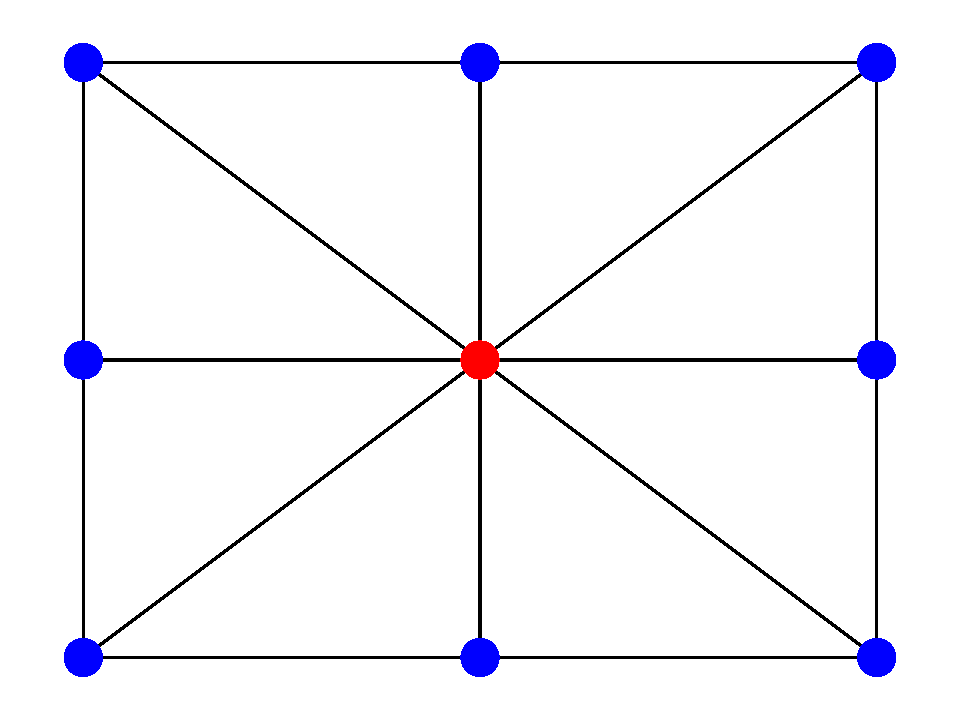
\includegraphics[width=0.5\textwidth]{figures/9pt_stencil_graph.pdf}<2->

  %     \null
  %     \null
  %     \null
  %     \null


  %   \column{0.5\textwidth}
  %     \begin{block}{Definition: 3D Stencil Interval Vertex Coloring (3DS-IVC)}<3->
  %       A problem where \( G \) is a 27-point \( 3D \) stencil, 
  %       composed of \(X \times Y \times Z\) vertices on a 3D grid such that two vertices 
  %       \( (i, j, k) \) and \( (i', j', k') \) are connected iff \( |i - i'| \leq 1 \), \( |j - j'| \leq 1 \), and
  %       \( |k - k'| \leq 1 \).
  %     \end{block}
  %     \centering
  %     \only<4->{%
  %       \animategraphics[loop,width=\textwidth, autoplay]{30}{figures/animation_27pt/output_}{0001}{180}
  %     }
  % \end{columns}
\end{frame}

% \begin{frame}{More Blocks}{theorem, proof}

  
%   \begin{theorem}
%     This is a theorem.
%   \end{theorem}
%   \begin{proof}
%     This is a proof.  Donec suscipit luctus lacus ut viverra. Proin molestie
%     eros tellus, vitae elementum nulla fringilla nec. Pellentesque facilisis,
%     elit ac egestas gravida, ante leo euismod velit, et suscipit est ex ut ex.
%   \end{proof}
% \end{frame}

\section{Heuristics}

\subsection{NP - Completeness}

\begin{frame}[fragile]{3DS-IVC $\in$ NP ?}
  \begin{overlayarea}{\textwidth}{\textheight}
    \only<1->{
      \begin{Lemma}<1->
        3DS-IVC $\in$ NP
      \end{Lemma}
    }
    
    \only<2->{
      \begin{block}{Proof.}
        \only<2->{
          Given a solution for 3DS-IVC, encoded with pairs of integers which are bounded between 0 and
          $\sum_{v \in V} w(v_i)$ $\mapsto$ are solutions in polynomial space. \\
        }
        \only<3->{
          Verify that no adjacent edges have overlapping intervals. $\forall (u, v) \in E:$
          \[ \left[ \text{{start}}(u), \text{{start}}(u) + w(u) \right) \cap \left[ \text{{start}}(v), \text{{start}}(v) + w(v) \right) = \emptyset. \]
        }
        \only<4->{
          Since $|E| \leq \frac{n(n-1)}{2}$ and checking if two intervals overlap is in $\mathcal{O}(1)$,
          the verification can be done in $\mathcal{O}(n^2)$ \qed.
        }
      \end{block}
    }
  \end{overlayarea}
\end{frame}

\begin{frame}{NAE-3SAT $\propto$ 3DS-IVC ?}
  \begin{block}{Idea of Proof}
    \begin{itemize}
      \onslide<1->{\item Construct an instance 3DS-IVC from an instance of NAE-3SAT in polynomial time. \\}
      \onslide<2->{\item Verify that a positive instance of NAE-3SAT results in a positive instance of 3DS-IVC.\\}
      \onslide<3->{\item Verify that if the created instance of 3DS-IVC is positive, then the instance of NAE-3SAT is also positive.\\}
      \onslide<4->{\item Since the 3DS-IVC problem is in NP and is harder than NAE-3SAT, which is an NP-Complete problem, 3DS-IVC is NP-Complete \qed.}
    \end{itemize}
  \end{block}
  
  \onslide<5->{
    The proof yields:
      \onslide<5->{
        \begin{theorem}
          Deciding whether a 27-pt stencil can be colored with less than $k$ colors is NP-Complete. \cite{main_paper}
        \end{theorem}
      }
  }
\end{frame}

\subsection{Algorithms}
\begin{frame}{Algorithms}
  1
\end{frame}



\section{Application and Experiments}
  \begin{frame}{Application and Experiments}

    In the application section I will probably cite \cite{kernel_estimation_1} and also \cite{kernel_estimation_2}.

  \end{frame}

\section{Footnotes}
\begin{frame}{Footnotes}
  You can also place footnotes, e.g.,
  here~\footnote{This is a footnote.}
  and here~\footnote{This is a longer footnote going over two lines.
    So I've added some more blah blah. Lorem ipsum whatever.}.
\end{frame}

\section{References}
\begin{frame}{References}

  \tiny\printbibliography
  
\end{frame}


\end{document}